\chapter{Deep Learning}
\label{ch:deep_learning}

\subsection{Biological neuron}
The human nervous system is the largest information processor in the human body. It is not the only information processor, but it is the largest and most efficient one. The human nervous system consists of several components. First, the brain, which is responsible for processing information and making decisions. Information to the brain comes from the senses along nerve fibers. The brain processes this information and decides how to react in a given situation. This solution is transmitted along the nerve fibers in the opposite direction to the muscles. This is how information is processed in the human body. The nervous system has several components. These components are responsible for different tasks. However, all of these components are made up of roughly the same cells called neurons.

A neuron is a component that makes up the entire human nervous system. Almost all neurons are structured roughly the same. 
So, a neuron has a neuron nucleus, which is also called the neuron body. An electrical charge is accumulated in the body of a neuron. From the body of the neuron there are many processes: there are small processes and large processes. The little outgrowths are so called dendrites. Through these processes, a signal from other neurons comes to our neuron. There is a large scion. This process is called an axon. A neuron transmits a signal to other neurons along the axon. The place where the axon of another neuron connects to the dendrites of our neuron is called a "synapse". The synapse is where the dendrite and axon meet. A synapse can be strong or it can be weak. If the synapse is strong, then the signal that is transmitted along the axon of the neuron will almost completely go to our neuron. If the synapse is weak, then practically no charge will cross from the axon of another neuron to our neuron. The synapse can change over time. Depending on the circumstances, the synapse can get stronger or it can get weaker. It is with the synapse tuning that the training of the biological neural network and, accordingly, the human nervous system is connected.

Considered visualization of the described above processes is as follows:
\begin{figure}[h]
    \centering 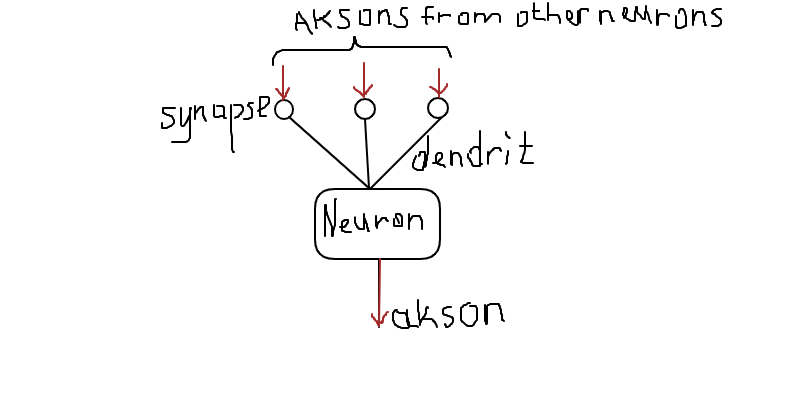
\includegraphics[width=7cm]{images/neuron_biological_model.png}
    \caption {biological model of neuron}
\end{figure}    

\subsection{Mathematical model of neuron}
Initially for simplicity we will represent neuron mathematical model graphically. It should be taken into consideration, the red characters denote tune parameters of the neuron.     
\begin{figure}[h]
    \centering 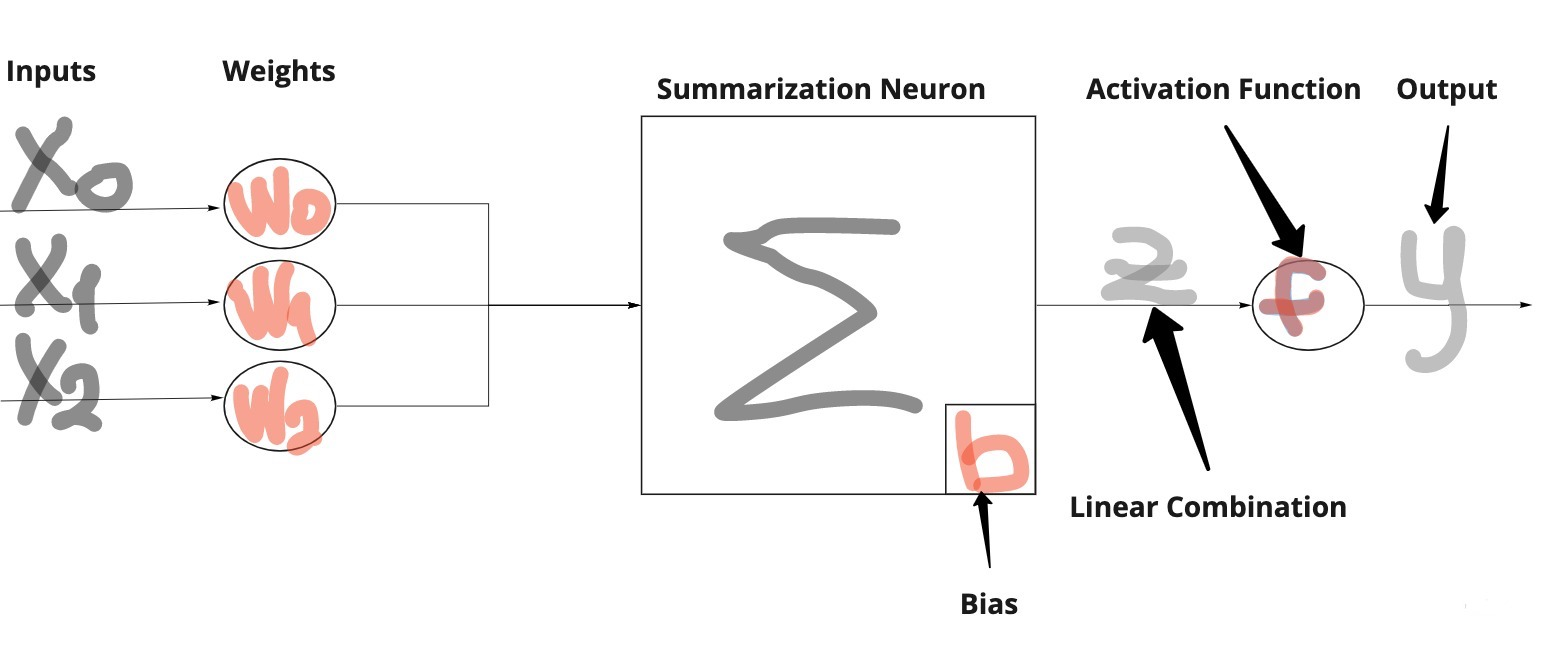
\includegraphics[width=7cm]{images/neuron_math_model.jpg}
    \caption {mathematical model of neuron}
\end{figure} 

In the mathematical model of the neuron, the body of the neuron, where the input signals accumulates, is denoted by a summarizing neuron. In addition, the biological neuron also has axons and dendrites, which get the inputs and send the outputs. Accordingly, in our mathematical model of the neuron, we will add inputs and outputs to the summarizing neuron. It's also worth keep in mind the biological neuron applies some actions with the signals that come into it, namely, it accumulates charge until it reaches some point and only after that forwards it further. This is what we will do in the mathematical model of the neuron using the activation functions.

Afterwards, let us mathematically define model of neuron as:
\[ y = f(z) = f(w_0*x_0+w_1*x_1+w_2*x_2+b) = f(\sum\limits_{i=0}^{N-1} w_i*x_i+b) = f(<\overrightarrow{w}, \overrightarrow{x}>+b) \]
Where:
\begin{itemize}
    \item $x_0, x_1, x_2$: inputs
    \item $w_0, w_1, w_2$: weights 
    \item $b$: some bias for increasing non-linearity   
    \item $f(z)$: some activation function 
\end{itemize}

Presently, let us see each component delicately.
Inputs can be either single number or vector of numbers. As for weights, we mainly should remember they are tuned parameters. Moreover it should be considered 2 potential situations to manage with. The first one is initialization of the weights. Here we have multiple options whereas we literally can define them either randomly or apply special initialisation techniques such as "He" initialization or "Xavier" initialization and others. The second situation we should be aware of is to somehow change the weights during model fitting, meaning weights should be changed in iterative manner from epoch to epoch. To do this we will apply backpropagation algorithm. Concerning the bias, which is like a weights, meaning tuned parameter, we can consider it allows to shift the activation function by adding a constant to the input of neuron. Hence, the last but not least component is activation function. In simplified terms, activation function is used to determine the output of neuron in a manner: "yes" or "no". It maps the resulting values in range between 0 to 1 or -1 to 1.            

To conclude, from the code base perspective one neuron functionality can be defined as:
\begin{lstlisting}
def _activation_function(weighted_sum):
  """step function is used as an example"""
  return 1 if weighted_sum > 0 else 0

def _neuron(inputs, weights, bias):
  weighted_sum = 0
  for input_vector, weight_vector, bias_vector in zip(inputs, weights, bias):
    particular_sum = (input_vector * weight_vector) + bias_vector
    weighted_sum += particular_sum
    output = _activation_function(weighted_sum)
  return output
\end{lstlisting}

      
\subsection{Activation function}
There is a significant number of various activation functions. Let us assume the very basic one named "step function" and figure out from general point of view how it works in both mathematical and geometrical conditions.   

The "step function" defined as:
\[ f(x) = \begin{cases} 0, & \mbox{if } x\mbox{ <= 0} \\ 1, & \mbox{if } x\mbox{ > 0} \end{cases} \]

The function has 2 strongly distinguished values: "0" and "1". The "spot" where the function changes it's value from "0" to "1" is named as dividing surface. Hence, the dividing surface "spot" is where the argument of activation function is equal "0".

\begin{figure}[h]
    \centering 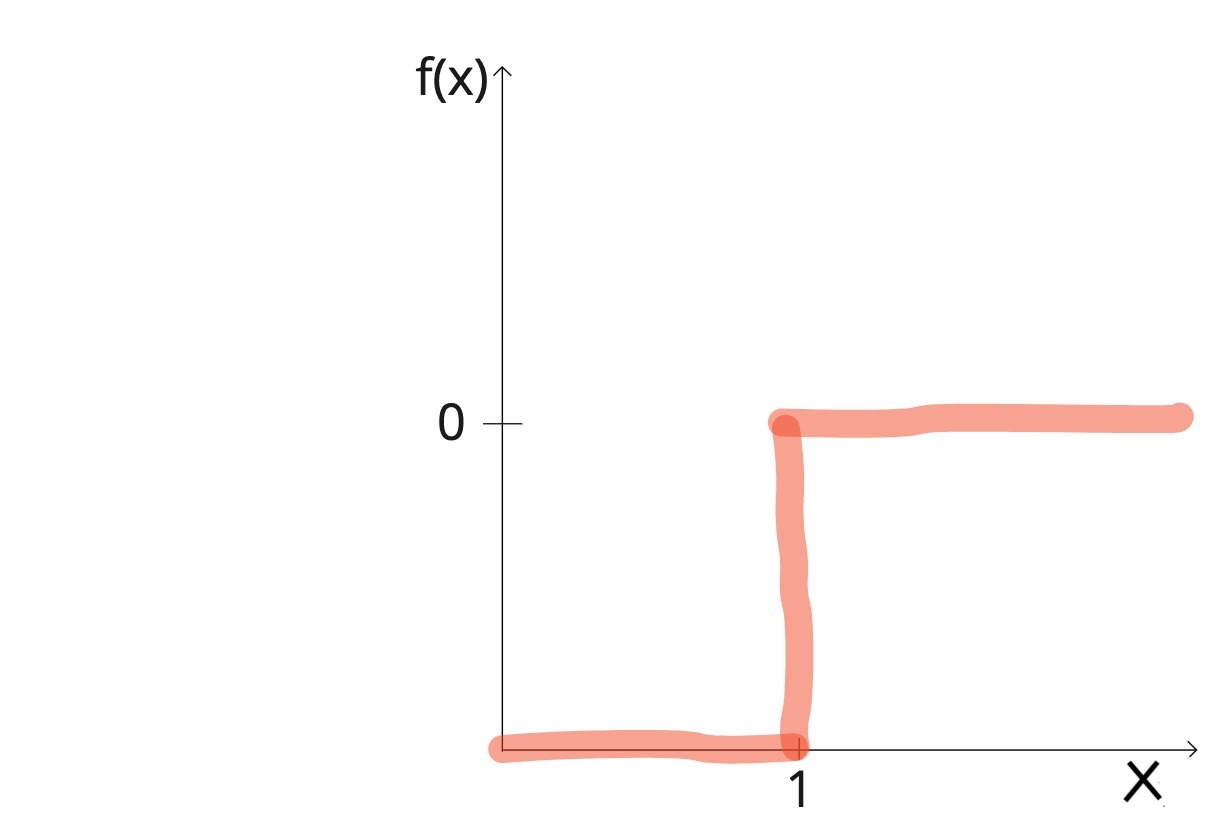
\includegraphics[width=7cm]{images/step_function.jpg}
    \caption {step function geometrical representation}
\end{figure}

The geometrical representation of step function can be derived as following. Assume there is the neuron formula:
\[ y = f(<\overrightarrow{w}, \overrightarrow{x}>+b) \]
The neuron does some linear operation, which is denoted by 2 parameters:
\begin{itemize}
    \item $\overrightarrow{w}$: vector of weights
    \item $b$: bias
\end{itemize}
Accordingly, the dividing surface is defined by following equitation which denotes equitation of straight line:
\[<\overrightarrow{w}, \overrightarrow{x}>+b = 0 \]

\begin{figure}[h]
    \centering 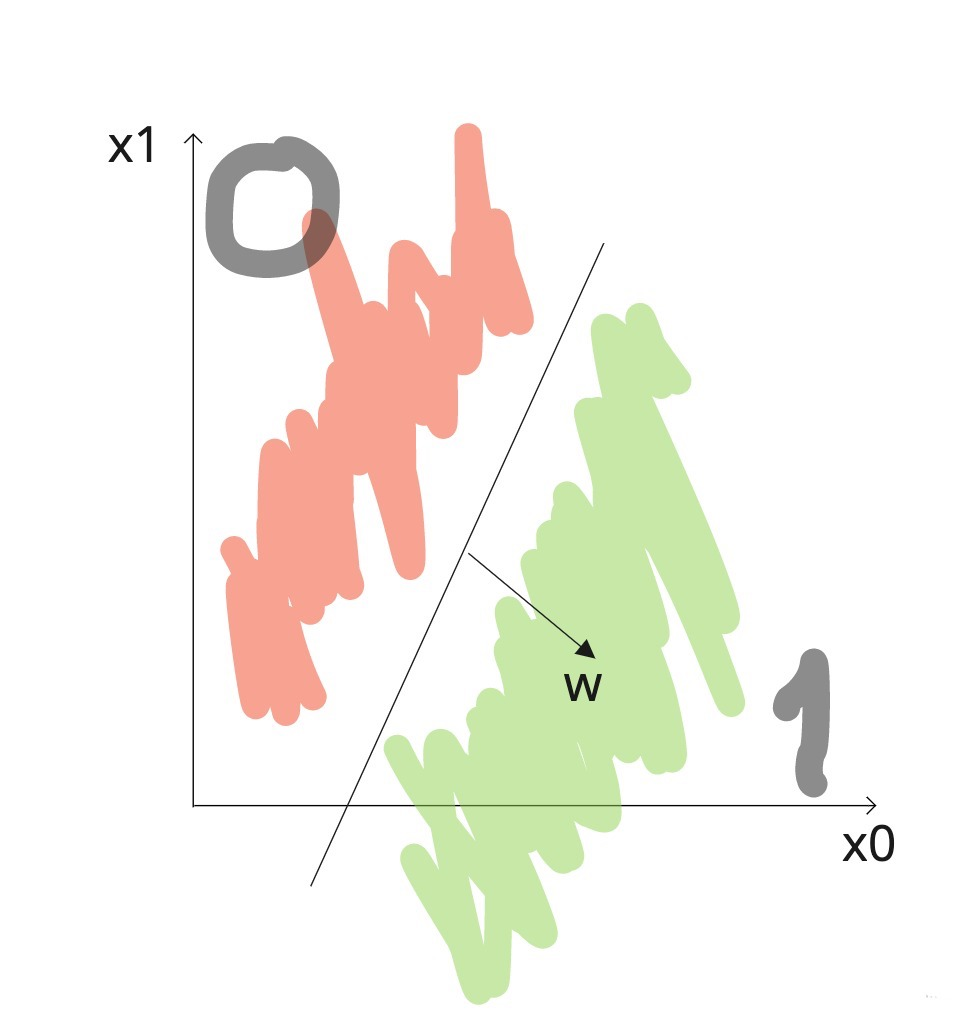
\includegraphics[width=7cm]{images/dividing_surface.jpg}
    \caption {dividing surface geometrical representation}
\end{figure}

From the one side the value of step function is equal "1" and from the other "0". The activation function is equal "1" that side of dividing surface where the vector "w" point out.

As for code base representation, step function can be defined as:
\begin{lstlisting}
def _step_function(weighted_sum):
  return 1 if weighted_sum >= 0 else 0
\end{lstlisting}
   
As it was mentioned earlier, step function is not the only one activation function. Let us proceed with other "sigmoid" activation function which unlike step function does not have discontinuity point at zero.
\begin{figure}[h]
    \centering 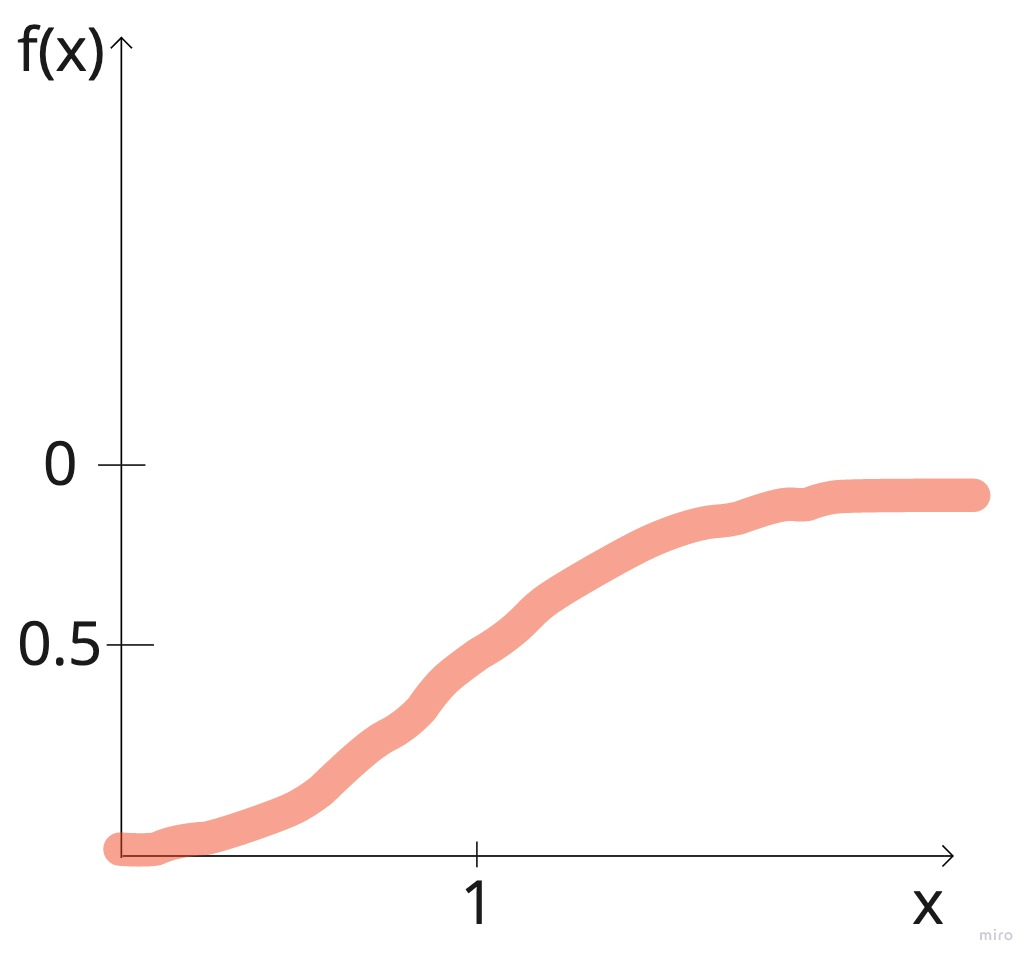
\includegraphics[width=7cm]{images/sigmoid_function.jpg}
    \caption {sigmoid activation function}
\end{figure}

The sigmoid activation function formed as:
\[ \sigma(x) = \dfrac{1}{1+e^x} \],

\[ \sigma(x) = \begin{cases} 1, & \mbox{if } x\mbox{$\xrightarrow{} + \infty$} \\ 0, & \mbox{if } x\mbox{$\xrightarrow{} - \infty$} \end{cases} \]

% ADD TANH, RELU ..
The list below points out the few rest functions which we will cover later on.

\subsection{From neuron to neural net}
So far we have discussed the properties and functional of a single neuron, which as a result outcomes a linear divide surface in geometrical terms. Meaning when we will concatenate the multiple neurons in some architecture we may achieve some nonlinear divide surfaces.
\begin{figure}[h]
    \centering 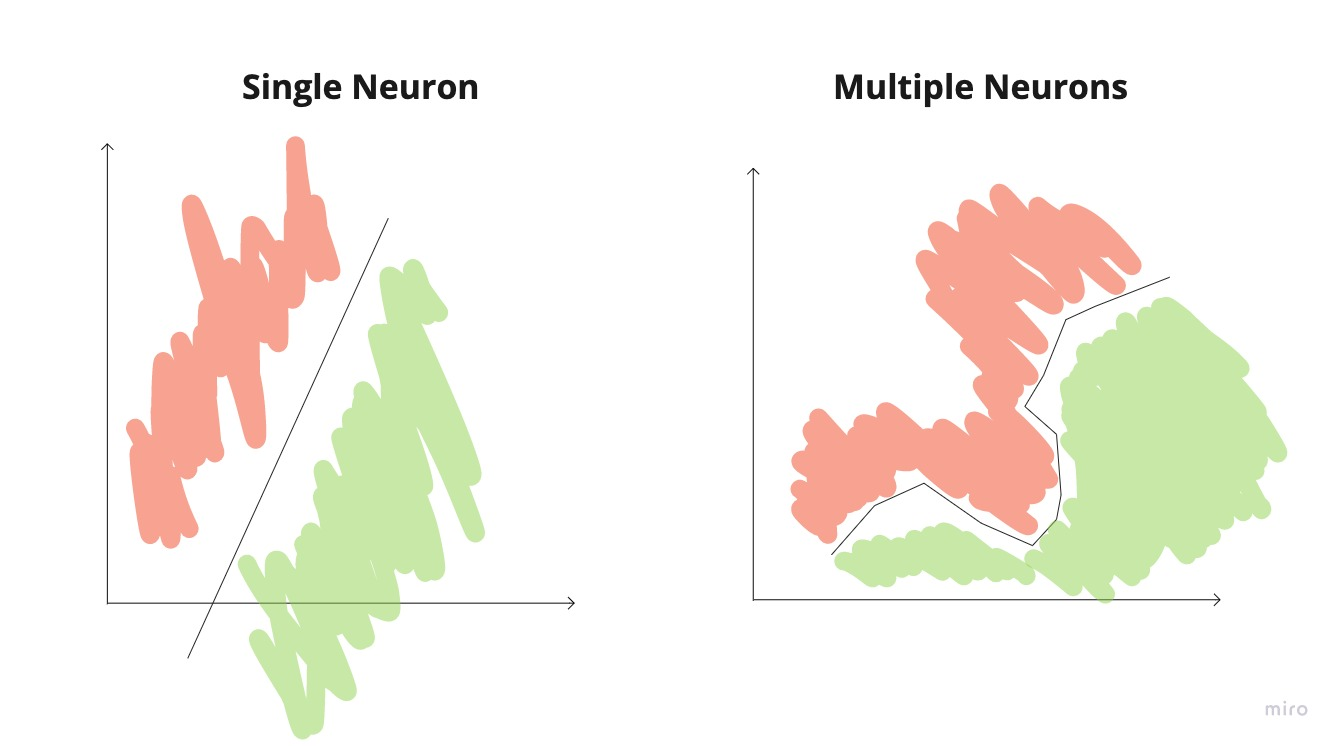
\includegraphics[width=7cm]{images/neuron_to_neural_net.jpg}
    \caption {single neuron surface vs multiple neurons surface}
\end{figure}

Now the question is how do we get the nonlinear dividing surface. Let us figure it out.
For simplicity define 3 neurons with linear activation function:
\begin{figure}[h]
    \centering 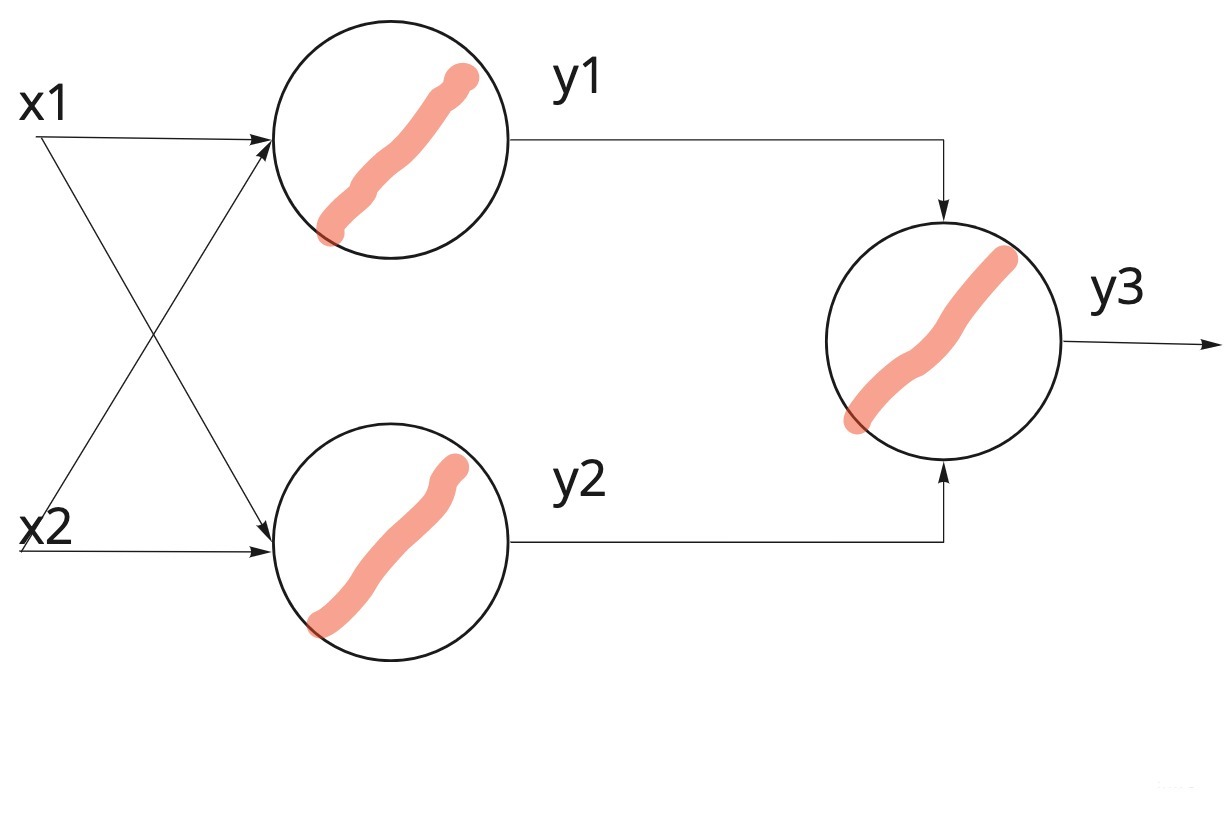
\includegraphics[width=7cm]{images/3_neurons_net.jpg}
    \caption {neural net with linear activation function}
\end{figure}
The results of performing the net can be considered as:
\[ y_3 = f(w_2^3*y_2+ w_1^3*y_1+b^3) = \]
By the reason $f$ is simple linear function, equation can be derived as:
\[ = w_2^3*y_2+ w_1^3*y_1+b^3 = \] 
\[ = w_2^3*f*(w_2^1*x_1+w_2^2*x_2+b^2) + w_1^3*f*(w_1^1*x_1+w_1^2*x_2+b^1) + b^3 = \]   
\[ = w_2^3*w_2^1*x_1+w_2^3*w_2^2*x_2+b^2 + w_1^3*w_1^1*x_1+w_1^3*w_1^2*x_2+b^1+ b^3 = \]
\[ = x_1[w_2^3*w_1^2 + w_1^3*w_1^1] + \]
\[   x_2[w_2^3*w_2^2 + w_1^3*w_2^1] + \]
\[   [w_2^3*b^2 + w_1^3*b^1 + b^3]  = \]
\[   x_1*\tilde{w_1} + x_2*\tilde{w_2} + \tilde{b} \]
Meaning the obtained result is just linear combination of inputs into the neural net. 


